% Messwerte: Alle gemessenen Größen tabellarisch darstellen
% Auswertung: Berechnung geforderter Ergebnisse mit Schritten/Fehlerformeln/Erläuterung/Grafik (Programme)
\section{Auswertung}
\label{sec:auswertung}


\subsection{Fehlerrechnung}
\label{sec:Fehlerrechnung}
Die Fehlerrechnung für die Bestimmung der Messunsicherheiten, wird mit Uncertainties \cite{uncertainties} gemacht.
Die Formel der Gauß Fehlerfortpflanzung ist gegeben durch
\begin{equation}
    \Delta f=\sqrt{\sum_{i=1}^N\left(\frac{\partial f}{\partial x_i}\right)^2 \cdot\left(\Delta x_i\right)^2}.
    \label{eqn:gauss}
\end{equation}
Für den Mittelwert bei $N$ Messwerten gilt 
\begin{equation}
    \bar{x} = \frac{1}{N}\sum\limits_{i = 1}^N x_i .
    \label{eqn:mittelwert}
\end{equation}
Der Fehler des Mittelwertes lässt sich berechnen mit
\begin{equation}
    \Delta \bar{x}=\frac{1}{\sqrt{N}} \sqrt{\frac{1}{N-1} \sum_{i=1}^N\left(x_i-\bar{x}\right)^2}.
    \label{eqn:mittelwertfehler}
\end{equation}
Zu Bestimmung der relativen Abweichung von den experimentellen Werten zu den theoretischen Werten wird die
Relation 
\begin{equation}
    \increment x = \frac{x_{exp}-x_{theo}}{x_{theo}}
\end{equation} 
genutzt.

\subsection{Bestimmung der Elementarladung}
\label{bestimmung der elementarladung}

Zunächst wird überprüft, ob die einzelenen Messwerte die Bedingung $2v_0 = v_{ab}-v_{auf}$ erfüllen.
Wenn die Messwerte die Relation nicht erfüllen und außerhalb des Rahmens der Messgenauigkeit sind, können 
diese verworfen werden. Verwendet werden die Werte, bei denen die prozentuale Abweichung vom Sollwert unter
$50 \%$ liegt. Die verwendbaren Messwerte und die berechneten Größen zur Bestimmung der Ladung werden in der \autoref{tab:tropfen_1} bis \autoref{tab:tropfen_17} dargestellt.


\begin{table}[H]
	\centering
	\captionsetup{width=0.95\linewidth}
	\caption{Ergebnisse für 1. Tröpfchen. Felder entsprechen jeweils primären, sekundären und tertiären Messgrößen. Hervorgehoben
			 ist der Mittelwert der Laufzeiten. Relative Abweichung zur Bedingung an Geschwindigkeit: $\protect\input{build/bed_1.tex}$.}
	\input{build/table_1.tex}
	\label{tab:tropfen_1}
\end{table}

\begin{table}[H]
	\centering
	\captionsetup{width=0.95\linewidth}
	\caption{Ergebnisse für 3. Tröpfchen. Felder entsprechen jeweils primären, sekundären und tertiären Messgrößen. Hervorgehoben
			 ist der Mittelwert der Laufzeiten. Relative Abweichung zur Bedingung an Geschwindigkeit: $\protect\input{build/bed_3.tex}$.}
	\input{build/table_3.tex}
	\label{tab:tropfen_3}
\end{table}

\begin{table}[H]
	\centering
	\captionsetup{width=0.95\linewidth}
	\caption{Ergebnisse für 4. Tröpfchen. Felder entsprechen jeweils primären, sekundären und tertiären Messgrößen. Hervorgehoben
			 ist der Mittelwert der Laufzeiten. Relative Abweichung zur Bedingung an Geschwindigkeit: $\protect\input{build/bed_4.tex}$.}
	\input{build/table_4.tex}
	\label{tab:tropfen_4}
\end{table}

\begin{table}[H]
	\centering
	\captionsetup{width=0.95\linewidth}
	\caption{Ergebnisse für 5. Tröpfchen. Felder entsprechen jeweils primären, sekundären und tertiären Messgrößen. Hervorgehoben
			 ist der Mittelwert der Laufzeiten. Relative Abweichung zur Bedingung an Geschwindigkeit: $\protect\input{build/bed_5.tex}$.}
	\input{build/table_5.tex}
	\label{tab:tropfen_5}
\end{table}

\begin{table}[H]
	\centering
	\captionsetup{width=0.95\linewidth}
	\caption{Ergebnisse für 6. Tröpfchen. Felder entsprechen jeweils primären, sekundären und tertiären Messgrößen. Hervorgehoben
			 ist der Mittelwert der Laufzeiten. Relative Abweichung zur Bedingung an Geschwindigkeit: $\protect\input{build/bed_6.tex}$.}
	\input{build/table_6.tex}
	\label{tab:tropfen_6}
\end{table}

\begin{table}[H]
	\centering
	\captionsetup{width=0.95\linewidth}
	\caption{Ergebnisse für 7. Tröpfchen. Felder entsprechen jeweils primären, sekundären und tertiären Messgrößen. Hervorgehoben
			 ist der Mittelwert der Laufzeiten. Relative Abweichung zur Bedingung an Geschwindigkeit: $\protect\input{build/bed_7.tex}$.}
	\input{build/table_7.tex}
	\label{tab:tropfen_7}
\end{table}

\begin{table}[H]
	\centering
	\captionsetup{width=0.95\linewidth}
	\caption{Ergebnisse für 8. Tröpfchen. Felder entsprechen jeweils primären, sekundären und tertiären Messgrößen. Hervorgehoben
			 ist der Mittelwert der Laufzeiten. Relative Abweichung zur Bedingung an Geschwindigkeit: $\protect\input{build/bed_8.tex}$.}
	\input{build/table_8.tex}
	\label{tab:tropfen_8}
\end{table}

\begin{table}[H]
	\centering
	\captionsetup{width=0.95\linewidth}
	\caption{Ergebnisse für 10. Tröpfchen. Felder entsprechen jeweils primären, sekundären und tertiären Messgrößen. Hervorgehoben
			 ist der Mittelwert der Laufzeiten. Relative Abweichung zur Bedingung an Geschwindigkeit: $\protect\input{build/bed_10.tex}$.}
	\input{build/table_10.tex}
	\label{tab:tropfen_10}
\end{table}

\begin{table}[H]
	\centering
	\captionsetup{width=0.95\linewidth}
	\caption{Ergebnisse für 12. Tröpfchen. Felder entsprechen jeweils primären, sekundären und tertiären Messgrößen. Hervorgehoben
			 ist der Mittelwert der Laufzeiten. Relative Abweichung zur Bedingung an Geschwindigkeit: $\protect\input{build/bed_12.tex}$.}
	\input{build/table_12.tex}
	\label{tab:tropfen_12}
\end{table}

\begin{table}[H]
	\centering
	\captionsetup{width=0.95\linewidth}
	\caption{Ergebnisse für 13. Tröpfchen. Felder entsprechen jeweils primären, sekundären und tertiären Messgrößen. Hervorgehoben
			 ist der Mittelwert der Laufzeiten. Relative Abweichung zur Bedingung an Geschwindigkeit: $\protect\input{build/bed_13.tex}$.}
	\input{build/table_13.tex}
	\label{tab:tropfen_13}
\end{table}

\begin{table}[H]
	\centering
	\captionsetup{width=0.95\linewidth}
	\caption{Ergebnisse für 14. Tröpfchen. Felder entsprechen jeweils primären, sekundären und tertiären Messgrößen. Hervorgehoben
			 ist der Mittelwert der Laufzeiten. Relative Abweichung zur Bedingung an Geschwindigkeit: $\protect\input{build/bed_14.tex}$.}
	\input{build/table_14.tex}
	\label{tab:tropfen_14}
\end{table}

\begin{table}[H]
	\centering
	\captionsetup{width=0.95\linewidth}
	\caption{Ergebnisse für 16. Tröpfchen. Felder entsprechen jeweils primären, sekundären und tertiären Messgrößen. Hervorgehoben
			 ist der Mittelwert der Laufzeiten. Relative Abweichung zur Bedingung an Geschwindigkeit: $\protect\input{build/bed_16.tex}$.}
	\input{build/table_16.tex}
	\label{tab:tropfen_16}
\end{table}

\begin{table}[H]
	\centering
	\captionsetup{width=0.95\linewidth}
	\caption{Ergebnisse für 17. Tröpfchen. Felder entsprechen jeweils primären, sekundären und tertiären Messgrößen. Hervorgehoben
			 ist der Mittelwert der Laufzeiten. Relative Abweichung zur Bedingung an Geschwindigkeit: $\protect\input{build/bed_17.tex}$.}
	\input{build/table_17.tex}
	\label{tab:tropfen_17}
\end{table}

Die verwendbaren Messwerte für die Zeiten $t_{\text{auf}}$ und $t_{\text{ab}}$ wurden gemittelt und der Fehler wurde nach
Gleichung \eqref{eqn:mittelwertfehler}bestimmt. Mit Hilfe des Python-Package Uncertainties \cite{uncertainties} wurden die Geschwindigkeiten der 
Teilchen berechnet. Als Wegstrecke $s$ wurde immer $(0.5 \pm 0.1) \cdot 10^{-3} \, \mathrm{m} $ angenommen. Um die Ladung der 
einzelnen Teilchen bestimmen zu können, wird die elektrische Feldstärke berechnet
\begin{equation*} 
    E = U/d,
\end{equation*}
wobei U der gemessenen Spannung entspricht und $d = (7.625 \pm 0.0051) \cdot 10^{-3}\,\mathrm{m} $ dem Abstand der Platten des Plattenkondensators.
Anhand der \autoref{fig:wider} und der \autoref{fig:graph} lässt sich über die gemessenen Thermistorwiderstände die Temperatur und die Viskosität bestimmen.

\begin{figure}[H]
    \centering
	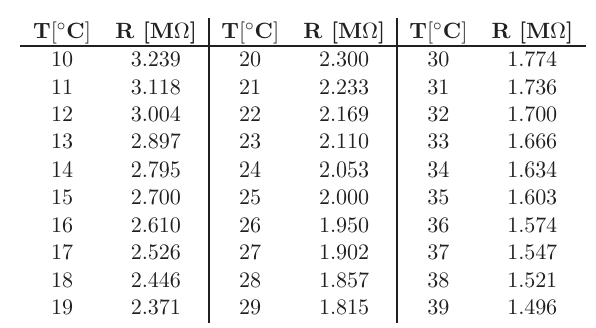
\includegraphics[width=0.75\linewidth]{content/grafik/widerstand.png}
	\captionsetup{width=0.925\linewidth}
	\caption{Thermistor-Widerstandstabelle.\cite{millikan}}
	\label{fig:wider}
\end{figure}

\begin{figure}[H]
    \centering
	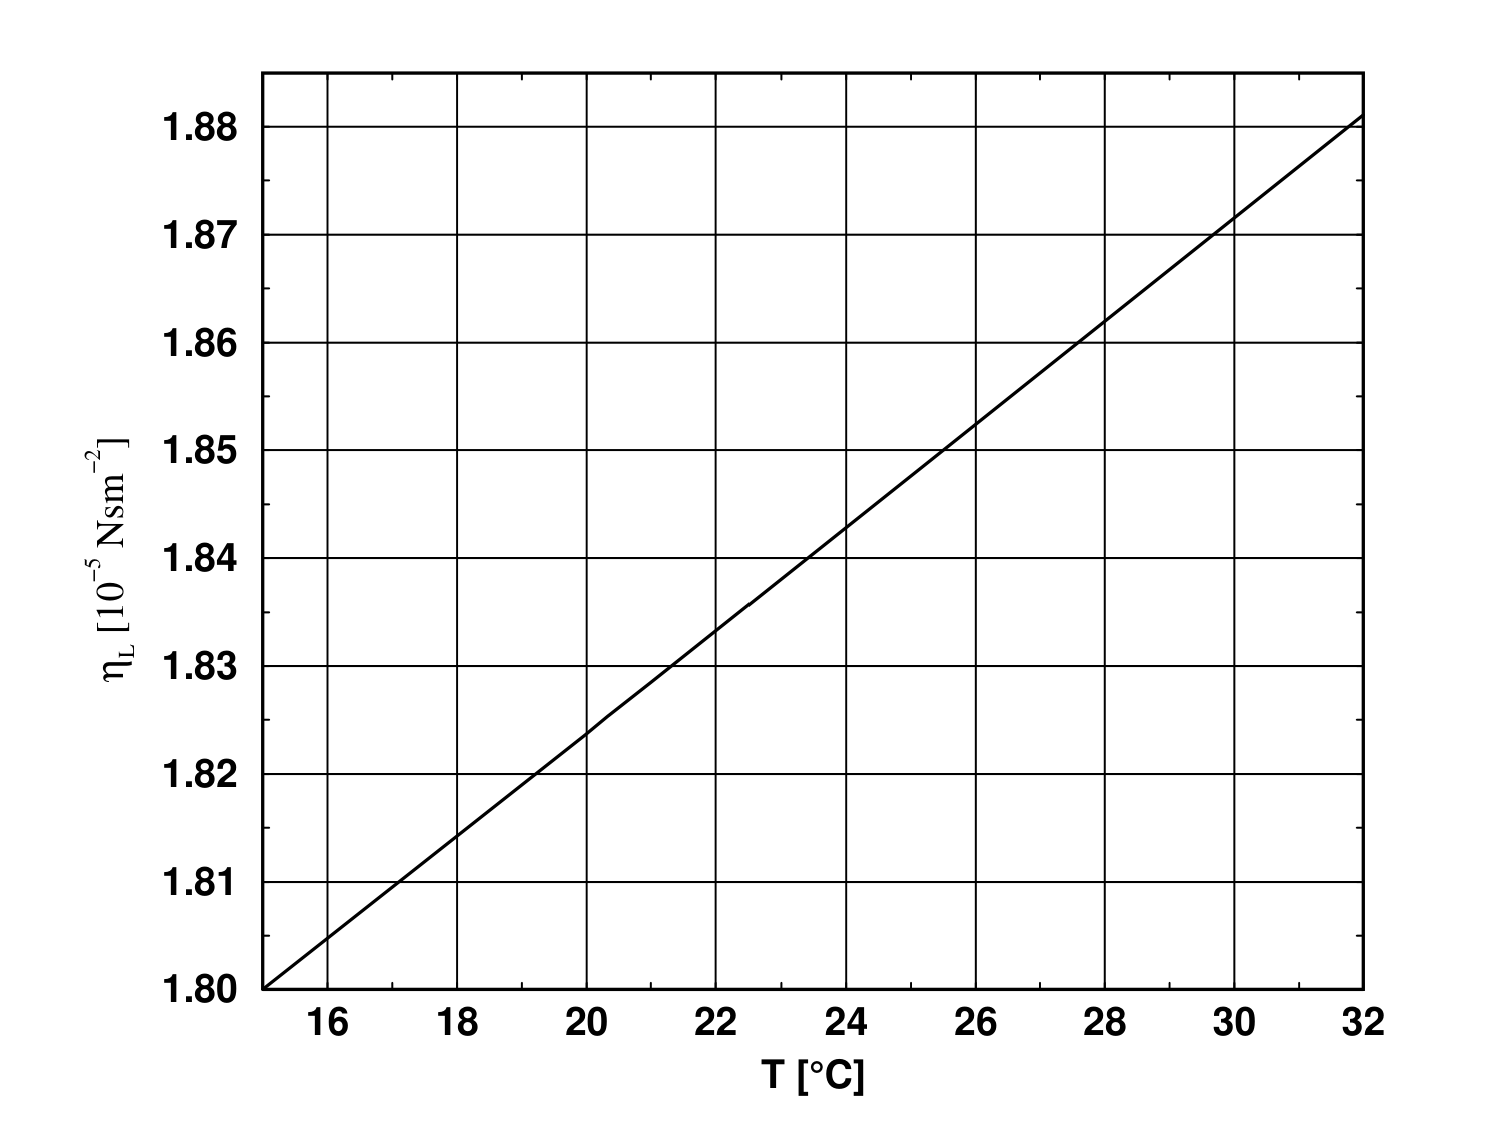
\includegraphics[width=0.75\linewidth]{content/grafik/graph.png}
	\captionsetup{width=0.925\linewidth}
	\caption{Viskosität von Luft als Funktion der Temperatur.\cite{millikan}}
	\label{fig:graph}
\end{figure}

Die abgelesenen Werte der Viskosität $\eta_L$ und der Temperatur $T$ wurden ebenfalls in den Tabellen der Tropfen aufgelistet.
Unter Verwendung der \autoref{eqn:radius_b} wird der Radius der Öltröpfchen bestimmt.
Daraufhin wird die unkorrigierte Ladung nach der \autoref{eqn:ladung} ermittelt, um anschließend 
über die \autoref{eqn:korrekt} die korrigierte Ladung der einzelnen Tropfen zu berechnen. Als Feldstärke $B$ war ein
Wert von $B = \qty{8.226e-3}{\pascal\meter}$ angegeben.

Die korrigierten Ladungen der Öltröpfchen wurden in der \autoref{fig:plot} zusammen mit ihren Fehlern dargestellt.

\begin{figure}[H]
    \centering
    \includegraphics[width=0.5\linewidth]{build/plot1.pdf}
    \caption{Histogramm der korrigierten Ladungen der Öltröpfchen}
    \label{fig:plot}
\end{figure}

In der \autoref{fig:plotkorr} wurden Gruppen eingeteilt, wobei eine Gruppe von Ladungen von Teilchen einem Vielfachen von der
gesuchten Elementarladung entspricht. Die Werte der Ladungen wurden in den eingezeichneten Gruppen gemittelt. Für die höchste
Stufe des ersten Teilchens ergibt das einen Wert von $ q_1 = (10 \pm 7) \cdot 10^{-19} \, \mathrm{C}$. Für die zweite Gruppe
lässt sich ein Wert von $q_2 = (6.0 \pm 1.9) \cdot 10^{-19} \, \mathrm{C}$ bestimmen. Bei der dritten Gruppe beträgt der gemittelte 
Wert der Ladungen $q_3 = (4.5 \pm 1.5) \cdot 10^{-19} \, \mathrm{C}$ und bei der Vierten $q_4 = (2.9 \pm 0.7) \cdot 10^{-19} \, \mathrm{C}$

\begin{figure}[H]
    \centering
    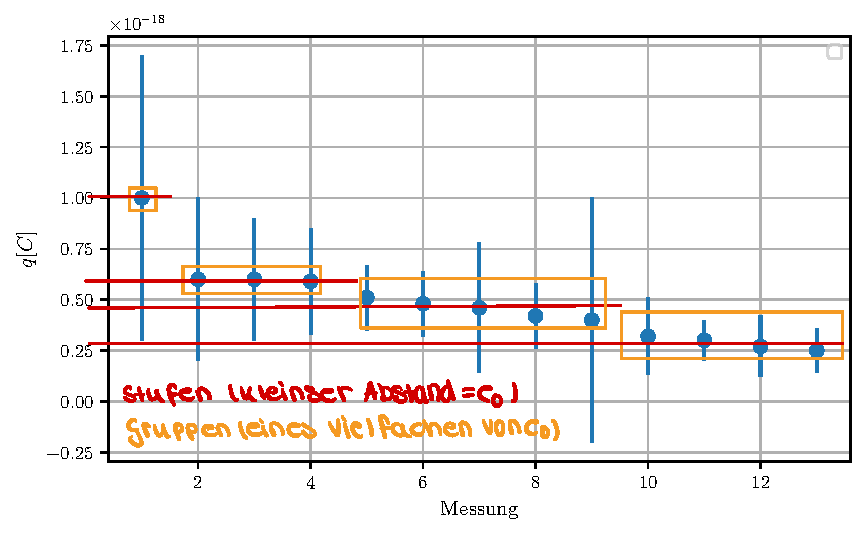
\includegraphics[width=0.5\linewidth]{content/grafik/plot1-korr.pdf}
    \caption{Histogramm der korrigierten Ladungen der Öltröpfchen}
    \label{fig:plotkorr}
\end{figure}

Die aus den eingteilten Gruppen bestimmten Ladungen ensprechen jeweils einem Vielfachen von $e$. Daraus kann geschlossen werden,
dass die Differenzen der Werte der unterschiedlichen Gruppen der Elementarladung entspricht. 
